\chapter{Sufficient Conditions for Stability}
\label{chap:suffcons}

We now turn to the discussion and proof of various analytic results in the pursuit of some conditions on the stability of \eqref{oseq}. Denote our eigenvalue $ c $ by
\begin{equation}
    c = c_r + i c_i.
\end{equation}

The real part $ c_r $ is commonly referred to as the \emph{wave speed} and the imaginary part $ c_i $ is referred to as the \emph{growth rate} \citep{drazin2004hydrodynamic}. The more interesting part in relation to instability is the growth rate $ c_i $ as if $ c_i > 0 $ then we have an unstable solution to \eqref{oseq}. However, it is also possible to find bounds on $ c_r $, though these do not provide any indication as to whether a type of flow is stable.

One of the first instances of this was \citet{synge1938hydrodynamical}, generalised by \citet{pai1954generalization}. Improvements were later made by \citet{joseph1968eigenvalue, joseph1969eigenvalue}.

\section{Equations for the wave speed and growth rate}

We begin by deriving equations for $ c_r $ and $ c_i $ in terms of integrals of $ \p $ and its derivatives as in \citet{synge1938hydrodynamical} and \citet{pai1954generalization}. \citet{pai1954generalization} derived these equations using generic boundary conditions. However, we will be using our more specific boundary conditions \eqref{osbc}.

Multiplying the Orr-Sommerfeld equation \eqref{oseq} by $ \phi_c $ (the complex conjugate of $ \phi $) and integrating with respect to $ z \in (-1, 1) $ we obtain the following equation:
\begin{gather}
    \inte{1}{-1}{(i \alpha R)^{-1} (D^2 - \alpha^2)^2 \phi \phi_c}{z}
    = \inte{1}{-1}{(U - c)(D^2 - \alpha^2) \phi \phi_c}{z} - \inte{1}{-1}{U'' \phi \phi_c}{z}.
\label{inteos}
\end{gather}

Throughout this chapter, we shall use the following notation to represent some commonly occurring integrals
\begin{align} 
        I^2_0 &= \inte{1}{-1}{\abs{\phi}^2}{z},\\
        I^2_1 &= \inte{1}{-1} {\abs{D \phi}^2}{z},\\
        I^2_2 &= \inte{1}{-1}{\abs{D^2 \phi}^2}{z}. 
\end{align}

As we will see later, there are inequalities on these integrals that help with finding bounds on $ c_i $ and $ c_r$. This means we would like to express our integral \eqref{inteos} in terms of these. We can already see some instances of these integrals appearing in our integral, for example, if we multiply out the brackets on the left-hand side we end up with the term $ (i \al R)^{-1} \al^4 \I{0} $. However, the terms containing $ (D^4 \phi) \phi_c $, $ (D^2 \p) \p_c $ and $ U (D^2 \p) \p_c $ require some manipulation to get in terms of $ \I{0},\ \I{1},\ \I{2}$. Our boundary conditions \eqref{osbc} can help with this! If we integrate by parts, they allow us to cancel out the evaluated integral term. This gives us the following results:

% To simplify this equation we need the following results obtained through integration by parts. Throughout the derivations, we will make extensive use of the boundary conditions of the Orr-Sommerfeld equation \eqref{oseq}, noting that they apply to $ \phi_c $ as well as $ \phi $. They allow us to cancel out many of the terms in our integration by parts. 

\begin{subequations}
    \begin{align}
        \inte{1}{-1}{(D^4 \phi) \phi_c}{z} &= \ieval{1}{-1}{(D^3 \phi) \phi_c} -\inte{1}{-1}{(D^3 \phi) (D \phi_c)}{z} \nonumber\\
        &= -\ieval{1}{-1}{(D^2 \phi)(D \phi_c)} + \inte{1}{-1}{(D^2 \phi)(D^2 \phi_c)}{z} = I^2_2, \\
        \inte{1}{-1}{(D^2 \phi) \phi_c}{z} &= \ieval{1}{-1}{(D \phi) \phi_c} - \inte{1}{-1}{(D \phi)(D \phi_c)}{z} = -I^2_1, \\
        \inte{1}{-1}{U (D^2 \phi) \phi_c}{z} &= \ieval{1}{-1}{(D \phi) U \phi_c} - \inte{1}{-1}{(D \phi)\qb{U' \phi_c + U (D \phi_c)}}{z} \nonumber\\ &= -\inte{1}{-1}{U' \qb{(D \phi)\phi_c + U (D \phi)(D \phi_c)}}{z},
    \end{align}
\end{subequations}

We have now represented most of the terms in our integral \eqref{inteos} in terms of $ \I{0},\ \I{1},\ \I{2}$, leaving us with
\begin{equation}
    (\I{2} + 2 \alpha \I{1} + \alpha^4 \I{0}) + i \alpha R Q = i \alpha c R (\I{1} + \alpha \I{0}),
\label{simpintos}
\end{equation}
where 
\begin{equation}
    Q = \inte{1}{-1}{U \abs{D \phi}^2 + (\alpha^2 U + U'') \abs{\phi}^2}{z} + \inte{1}{-1}{U' (D \phi) \phi_c}{z}.
\end{equation} 

To get separate equations for $ c_i $ and $ c_r $ we need to split \eqref{simpintos} into real and imaginary parts. All of the integrals $ \I{0},\ \I{1},\ \I{2}$ are real, meaning that the only things we need to calculate are the real and imaginary parts of $Q $. Taking the real part of $ Q $:
\begin{align}
    \Re{Q} = \tfrac{1}{2}(Q - Q_c) = \tfrac{1}{2} \inte{1}{-1}{&U \abs{D \phi}^2 + \alpha^2 U + U'') \abs{\phi}^2}{z} \nonumber\\
    &+ \tfrac{1}{2} \inte{1}{-1}{U' \qb{(D \phi) \phi_c + \phi (D \phi_c)}}{z}.
\end{align}
We can simplify this a bit if we note that $ D(\phi \phi_c) = (D \phi) \phi_c + \phi (D \phi_c) $ and integrate by parts, leading to
\begin{align}
    \Re{Q} &= \inte{1}{-1}{U \abs{D \phi}^2 + \alpha^2 U + U'') \abs{\phi}^2}{z} + \tfrac{1}{2} \qb{\ieval{1}{-1}{U' \phi \phi_c} - \inte{1}{-1}{U'' \phi \phi_c}{z}} \nonumber\\
    &= \inte{1}{-1}{U \abs{D \phi}^2 + \alpha^2 U + U'') \abs{\phi}^2}{z} - \tfrac{1}{2}\inte{1}{-1}{U'' \phi \phi_c}{z} \nonumber\\ 
    &= \inte{1}{-1}{U \abs{D \phi}^2 + \alpha^2 U + \tfrac{1}{2} U'') \abs{\phi}^2}{z}.
    \label{reQ}
\end{align}

For the imaginary part of $Q$, we have
\begin{align}
    \Im{Q} &= \tfrac{1}{2i} (Q - Q_c) = \tfrac{1}{2i} \inte{1}{-1}{U' \qb{(D \phi) \phi_c - \phi (D \phi_c)}}{z} \nonumber\\ 
    &= \tfrac{1}{2} i \inte{1}{-1}{U' \qb{(D \phi_c) \phi - \phi_c (D \phi)}}{z}.
\label{imQ}
\end{align}

Now we can split our integral into real and imaginary parts as follows
\begin{align}
    \alpha R \Re{Q} &= - \alpha R c_r (\I{1} + \alpha^2 \I{0}), \\
    -\alpha R \Im{Q} + (\I{2} + 2 \alpha^2 \I{1} + \alpha^4 \I{0}) &= -\alpha R c_i (\I{1} + \alpha \I{0}).
\end{align}

Rearranging these gives us our equations for $ c_i $ and $ c_r$
\begin{subequations}
    \begin{align}
        c_r &= \frac{\Re{Q}}{\I{1} + \alpha^2 \I{0}}, \label{c_r} \\
        c_i &= \frac{(\Im{Q} - (\alpha R)^{-1} (\I{2} + 2 \alpha^2 \I{1} + \alpha^4 \I{0}))}{\I{1} + \alpha^2 \I{0}}. \label{c_i}
\end{align}    
\end{subequations}

We now have equations for both the wave speed $ c_r $ and the growth rate $ c_i $. This chapter will now turn to proving various results and bounds on both quantities.

First though, we should introduce those bounds on $ \I{0},\ \I{1},\ \I{2} $ that were mentioned earlier. It can be shown that the following lemma holds:

\begin{lemma}[\citet{joseph1968eigenvalue, joseph1969eigenvalue}]
Let $ \phi \in \Bar{H}(\al) $. Then
\begin{subequations}
\begin{align}
    \I{1} \geq \lambda^2_1(\al) \I{0} ,\ \ \I{2} \geq \lambda^2_2(\al) \I{1},\ \ \I{2} \geq \lambda^2_3 (\al) \I{0}, \label{jineq1} \\ 
    \lambda^2_1(\al) \geq \tfrac{1}{4} \pi^2 ,\ \ \lambda^2_2(\al) \geq \pi^2, \ \ \lambda^2_3 \geq (\frac{4.73}{2})^4,  \label{jineq2}
\end{align}
\label{lamineq}
\end{subequations}
with equality in \eqref{lamineq} when $ \al = 0 $.
\label{josephlemma}
\end{lemma}

\proof An outline of the proof of this lemma is given here. The reader is encouraged to read \citet{joseph1969eigenvalue} for more details. 

$ \lambda_1,\ \lambda_2,\ \lambda_3$ are derived from the following minimum problems,
\begin{align}
    \lambda_1^2 &= \min \frac{\inte{1}{0}{(\p')^2}{z} + \al \p(1)^2}{\inte{1}{0}{\p^2}{z}} = \min \frac{\Tilde{\I{1}}}{\Tilde{\I{0}}}, \\
    \lambda_2^2 &= \min \frac{\inte{1}{0}{(\p'')^2}{z} }{\inte{1}{0}{(\p')^2}{z}  + \al \p(1)^2} = \min \frac{\Tilde{\I{2}}}{\Tilde{\I{1}}}, \\
    \lambda_3^2 &= \min \frac{\inte{1}{0}{(\p'')^2}{z} }{\inte{1}{0}{\p^2}{z}} = \min 
 \frac{\Tilde{\I{2}}}{\Tilde{\I{0}}}.
 \label{minimumproblems}
\end{align}

The tilde over the $ \I{i}$ in these minimum value problems are to indicate that these are the $ \I{i}$ defined by Joseph.

To minimise these, Joseph considers the Euler-Lagrange equations and finds from here that $ \lambda_1 $ comes from the smallest positive root of the equation 
\begin{equation}
    \lambda \cos \lambda + \al \sin \lambda = 0.
\end{equation}

$ \l_2$, $ \l_3$ are the smallest positive roots of the following determinants
\begin{align}
    \begin{vmatrix}
        \l_2 (\cos \l_2 - 1) + \al \sin \l_2 - \al \l_2 & - \l_2 \sin \l_2 + \al (\cos \l_2 - 1) \\
        -\l_2 \cos \l_2 - \al \sin \l_2 & \l_2 \sin \l_2 - \al \cos \l_2
    \end{vmatrix} &= 0, \\
    \begin{vmatrix}
        \l_3 ( \cosh \l_3 - \cos \l_3 ) + \al ( \sinh \l_3 - \sin \l_3) & \\
         & \l_3 ( \sinh \l_3 + \sin \l_3 ) + \al ( \cosh \l_3 - \cos \l_3) \\
        \l_3 ( \cosh \l_3 + \cos \l_3 ) + \al ( \sinh \l_3 + \sin \l_3) & \\ & \l_3 ( \sinh \l_3 - \sin \l_3 ) + \al ( \cosh \l_3 + \cos \l_3)
    \end{vmatrix} &= 0.
\end{align}

All of these equations come from the boundary conditions that must be satisfied by the eigenfunctions of the Euler-Lagrange equations. 

However, as mentioned before, Joseph defines his $ \I{i} $ differently from us. His definitions have boundary conditions on $ z = 0, z = 1$ unlike our boundary conditions on $ z = -1, z = 1$, and his definition for $ \I{1}$ includes the term $ \al \p(1)^2$. So why can we use this lemma in our case? 

Consider the transformation $ y = (1 + z) / 2$ which maps $ z $ to a range of $ y $ between $ 0 $ and $ 1$, the same as Joseph and set $ \al = 0 $ in $ \Tilde{\I{1}}$. If we apply this to our definition of $ \I{0},\ \I{1},\ \I{2} $ we get the following
\begin{align}
    \I{0} &= 2 \Tilde{\I{0}}, \\
    \I{1} &= 2 \Tilde{\I{1}}, \\
    \I{2} &= 2 \Tilde{\I{2}}.
\end{align}

When we substitute these into the minimum problems considered by Joseph \eqref{minimumproblems} the factors cancel out, showing that our definitions for $ \I{i}$ satisfy Lemma \ref{josephlemma} with $ \al = 0$. This means that the second set of inequalities \eqref{jineq2} become equalities and the first set of inequalities \eqref{jineq1} become
\begin{equation}
    \I{1} \geq \tfrac{1}{4} \pi^2 \I{0} ,\ \ \I{2} \geq \pi^2 \I{1},\ \ \I{2} \geq (\tfrac{4.73}{2})^4 \I{0}.
\end{equation}

We can now use these inequalities along with equations \eqref{c_i} and \eqref{c_r} to find bounds on $ c_r$ and $ c_i$.

\section{Bounds on the wave speed}
Let us first discuss the wave speed $ c_r $. While this quantity does not tell us anything about stability, it can be shown that it is still bounded \citep{synge1938hydrodynamical, pai1954generalization, joseph1968eigenvalue, joseph1969eigenvalue}, which confines $ c $ to a strip in the complex plane. Let us begin by proving the result given by \citet{pai1954generalization}.

\citet{pai1954generalization} showed that:
\begin{equation}
    \frac{U''_{min}}{2 \al^2} + U_{min} < c_r < \frac{U''_{max}}{2 \al^2} + U_{max}.
    \label{paicr}
\end{equation}

\proof
Rearrange \eqref{c_r} to get
\begin{equation}
    \inte{1}{-1}{(U - c_r) \abs{D \phi}^2}{z} + \al^2 \inte{1}{-1}{\qb{(U - c_r) + \frac{U''}{2 \al^2}}\abs{\phi}^2}{z} = 0.
\end{equation}

The argument for obtaining \eqref{paicr} is as follows. Assume $ U $ is positive. Now if $ c_r < 0$ then the first integral must be positive which means that the second integral must be negative. This means that
\begin{gather}
    (U - c_r) + \frac{U''}{2 \al^2} < 0 \text{ for some } z \in (-1, 1) \nonumber\\
    \implies c_r > \frac{U''_{min}}{2 \al^2} + U_{min}. 
\end{gather}

If $ c_r > 0 $ and $ c_r \geq U_{max} $ then the first integral is negative which means that the second integral must be positive. This means that
\begin{gather}
    (U - c_r) + \frac{U''}{2 \al^2} > 0 \text{ for some } z \in (-1, 1) \nonumber\\
    \implies c_r < \frac{U''_{max}}{2 \al^2} + U_{max}. 
\end{gather}

Combining these inequalities gives \eqref{paicr}. Note that if $ U $ is assumed negative then the same argument follows with the inequalities derived for the opposite case. This means that \eqref{paicr} is true for any $ U $ as any $ U $ can be split into regions of positive and negative for which the appropriate argument can be applied.

For plane Couette flow we have that $ U'' = 0 $ which leaves us with
\begin{equation}
    U_{min} < c_r < U_{max}.
\end{equation}

For plane Poiseuille flow we have that $ U_{min} = 0 $, $ U''_{max} = 0 $ which gives
\begin{equation}
    \frac{U''_{min}}{2 \al^2} < c_r < U_{max}.
\end{equation}

In our case, with the range $ -1 \leq z \leq 1 $ we have that for Couette flow
\begin{equation}
    -1 < c_r < 1,
\end{equation}
and for Poiseuille flow
\begin{equation}
    \frac{-1}{\al^2} < c_r < 1.
\end{equation}

This result was improved by \citet{joseph1968eigenvalue, joseph1969eigenvalue} who proved

\begin{theorem}[\citet{joseph1969eigenvalue} Theorem 2] 
Let $C(\al, R)$ be any eigenvalue of \eqref{oseq}. Then the following holds:
\begin{outline}
    \1 $ U''_{min} \geq 0: $
        \2 $ U_{min} < c_r < U_{max} + \frac{2 U''_{max}}{\pi^2 + 4 \al^2}; $
    \1 $ U''_{min} < c_r < U_{max}: $
        \2 $ U_{min} + \frac{2 U''_{min}}{\pi^2 + 4 \al^2} < c_r < \frac{2 U''_{max}}{\pi^2 + 4 \al^2} $
    \1 $ U''_{max} \leq 0: $
        \2 $ U_{min} + \frac{2 U''_{min}}{\pi^2 + 4 \al^2} < c_r < U_{max} $
\end{outline}
\end{theorem}

\begin{proof}
From \eqref{c_r} we have that 
\begin{align*}
    c_r &= \frac{(U(a) + \al^2 U(a)) \I{0} + \tfrac{1}{2} U''(b) \I{0}}{\I{1} + \al^2 \I{0}} \nonumber\\
    &= \frac{(U(a) + \al^2 U(a)) \I{0} + \tfrac{1}{2} U''(b) \I{0}}{\I{1} + \al^2 \I{0}} \nonumber\\
    &= U(a) + \frac{U''(b)}{2(\tfrac{\I{1}}{\I{0}} + \al^2)},
\end{align*}
where $ a $ and $ b $ represent the mean values of $ U $ and $ U'' $ respectively (in the range $ (-1, 1) $). For the remainder of the proof, we use the fact that $ \frac{\I{1}}{\I{0}} \geq \tfrac{1}{4} \pi^2 $ (given in \eqref{lamineq}) plus the fact that $ U_{min} < U(a) < U_{max} $ (by definition) in each of the 3 cases:
\begin{outline}
    \1 $ U''_{min} \geq 0: $
        \2  $ \implies 0 < \frac{U''(b)}{\tfrac{\I{1}}{\I{0}} + \al^2} < \frac{U''_{max}}{\tfrac{1}{4} \pi^2 + \al^2} $
        \2 $ \implies U_{min} < c_r < U_{max} + \frac{2 U''_{max}}{\pi^2 + 4 \al^2} $.
    \1 $ U''_{min} < c_r < U_{max}: $
        \2 $ \implies \frac{U''_{min}}{\tfrac{1}{4} \pi^2 + \al^2} < \frac{U''(b)}{\tfrac{\I{1}}{\I{0}} + \al^2} < \frac{U''_{max}}{\tfrac{1}{4} \pi^2 + \al^2} $
        \2 $ \implies U_{min} + \frac{2 U''_{min}}{\pi^2 + 4 \al^2}< c_r < \frac{2 U''_{max}}{\pi^2 + 4 \al^2} $.
    \1 $ U''_{max} \leq 0: $
        \2 $ \implies \frac{U''_{min}}{\tfrac{1}{4} \pi^2 + \al^2} < \frac{U''(b)}{\tfrac{\I{1}}{\I{0}} + \al^2} $
        \2 $ \implies U_{min} + \frac{2 U''_{min}}{\pi^2 + 4 \al^2}< c_r < U_{max} $.
\end{outline}
\end{proof}

For Poiseuille flow between $ -1 < z < 1 $, we have that $ U'' = -2 $, which means that case 3 of the above is satisfied. This leaves us with the following bounds for $ c_r $:
\begin{equation}
    \frac{-4}{\pi^2 + 4 \al^2} < c_r < 1.
\end{equation}

In the case of Couette flow, we have that $ U'' = 0 $, which means that cases 1 and 3 are satisfied. This may seem like an issue, but they both give the same bounds on $ c_r$, 
\begin{equation}
    -1 < c_r < 1.
\end{equation}

Notice that these are the same as the bounds given by Pai, so in the case of Couette flow, Joseph's bounds don't offer any improvement. However, if we consider the mode with $ \al = 1 $ in the case of Poiseuille flow, then Joseph's bounds are an improvement. Notice that in both cases, as $ \al \to \infty$, $ c_r $ is found in the range $ 0 $ to $ 1 $, whereas for Couette flow, $ c_r $ is found in the range $ -1 $ to $ 1$.

Both these results limit $ c_r $ to strips in the complex plane. However, they don't give us any direct results relating to stability. For that, we now turn to the growth rate $ c_i $.

\section{Bounds on the growth rate}

The growth rate is important because a state cannot be stable if $ c_i > 0 $ for any eigenvalue of \eqref{oseq}. This is because if we look at our streamfunction solution \eqref{streamfunction} we can see that any solutions with $ c_i > 0 $ will blow up as $ t $ increases, while any with $ c_i < 0$ will decay, implying they are stable. $ c_i > 0 $ is therefore generally taken as the \emph{criterion for instability}. We will begin this section by deriving \citet{synge1938hydrodynamical} results and will follow by deriving the improvements made by \cite{joseph1968eigenvalue, joseph1969eigenvalue}.

The first result we need is that the following inequality holds
\begin{equation}
    \abs{\Im{Q}} \leq q I_1 I_0,
\end{equation}
where $ q = U'_{max}$ and
\begin{equation}
    I_1 = \inte{1}{-1}{D \phi}{z},\ \ I_0 = \inte{1}{-1}{\phi}{z}.
\end{equation}

\begin{proof}
We have that from \eqref{imQ}
\begin{equation}
    \abs{\Im{Q}} = \tfrac{1}{2} \inte{1}{-1}{\abs{U' ( \phi ( D \phi_c) - (D \phi) \phi_c)}}{z}.
\end{equation}

From repeated uses of Schwarz's Inequality, we get the following
\begin{align}
    \abs{\Im{Q}} &\leq \inte{1}{-1}{\abs{U'} \abs{\tfrac{1}{2} ( \phi (D \phi_c) - (D \phi) \phi_c)}}{z} \nonumber\\
    &\leq \inte{1}{-1}{\abs{U'} \abs{D \phi \phi_c}}{z} \nonumber\\
    &\leq \inte{1}{-1}{\abs{U'} \abs{D \phi} \abs{\phi_c}}{z} = \inte{1}{-1}{\abs{U'} \abs{D \phi}{\phi}}{z} \nonumber\\
    &\leq \inte{1}{-1}{\abs{U'}}{z} I_1 I_0 \nonumber\\
    &\leq U'_{max} I_1 I_0 = q I_1 I_0.
\end{align}
\end{proof} 

Using this inequality in \eqref{c_i} gives us the following important result
\begin{equation}
        c_i \leq \frac{(q I_1 I_0 - (\alpha R)^{-1} (\I{2} + 2 \alpha^2 \I{1} + \alpha^4 \I{0}))}{\I{1} + \alpha^2 \I{0}}.
\label{c_iineq}
\end{equation}

For stability, $ c_i < 0 $. This means the following inequality holds
\begin{equation}
    \frac{(q I_1 I_0 - (\alpha R)^{-1} (\I{2} + 2 \alpha^2 \I{1} + \alpha^4 \I{0}))}{\I{1} + \alpha^2 \I{0}} < 0.
\label{stabineq}
\end{equation}

We can rearrange the above to obtain the following result given by \citet{joseph1968eigenvalue}
\begin{equation}
    \al R q < \frac{\I{2} + 2 \al^2 \I{1} + \al^4 \I{0}}{I_1 I_0}.
\label{jaRq}
\end{equation}

\citet{synge1938hydrodynamical} now proves the following results combined into one theorem in \citet{joseph1968eigenvalue}). Note these are derived in the range $ z \in (-1, 1) $.

\begin{theorem}[\citet{synge1938hydrodynamical} condition for stability]
No amplified disturbances of \eqref{oseq} exist if 
\begin{equation}
    \al R q < \max[A_1, A_2, A_3],
\end{equation}
where 
\begin{align}
    A_1 &= 2^{\tfrac{3}{2}} \al^2 (\al^2 + 1)^{\tfrac{1}{2}}, \nonumber\\
    A_2 &= (2 \al^2 + 1)^{\tfrac{1}{2}}(4 \al^4 + 1)^{\tfrac{1}{2}}, \nonumber\\
    A_3 &= 2^{\tfrac{3}{2}} \al (1 - \al^2 + \al^3 + \al^4)^{\tfrac{1}{2}}.
    \label{sbounds}
\end{align}
\end{theorem}

\begin{proof}
    To begin, we consider the following integral
    \begin{align}
        \inte{1}{-1}{(\phi + a z \phi' &+ b \phi'')(\phi_c + a z \phi_c' + b \phi''_c)}{z} \nonumber\\
        = \I{0} &+ \inte{1}{-1}{a z \phi \phi_c' + b \phi \phi''_c + a z \phi' \phi_c + a^2 z^2 \abs{\phi'}^2 \nonumber\\ &+ a b z \phi' \phi''_c + b \phi'' \phi_c + a b z \phi'' \phi'_c}{z} + b^2 \I{2} \nonumber\\
        = \I{0} &+ a \inte{1}{-1}{z (\phi \phi'_c + \phi' \phi_c)}{z} + b \inte{1}{-1}{\phi \phi''_c + \phi'' \phi_c}{z} \nonumber\\
        &+ a^2 \inte{1}{-1}{z^2 \abs{\phi'}^2}{z} + ab \inte{1}{-1}{z (\phi' \phi''_c + \phi'' \phi'_c)}{z} + b^2 \I{2} > 0.
        \label{phiresult}
    \end{align}

    We now want to express some of the more 'messy' integrals in the above as $ \I{2}, \I{1}, \I{0} $. Using the boundary conditions and the fact that 
    \begin{align}
        (\phi \phi_c)' &= \phi \phi'_c + \phi' \phi_c, \nonumber\\
        (\phi' \phi_c')' &= \phi' \phi''_c + \phi'' \phi'_c,
    \end{align} 
    we have
    \begin{equation}
        \inte{1}{-1}{z (\phi' \phi''_c + \phi'' \phi'_c)}{z} = \ieval{1}{-1}{z (\phi' \phi'_c)} - \inte{1}{-1}{\phi' \phi'_c}{z} = - \I{1},
    \end{equation}
    also
    \begin{align}
        \inte{1}{-1}{z (\phi \phi'_c + \phi' \phi_c)}{z} = \ieval{1}{-1}{z \phi \phi_c} - \inte{1}{-1}{\phi \phi_c}{z} = -\I{0}, 
    \end{align}
    and
    \begin{align}
        \inte{1}{-1}{\phi \phi''_c + \phi'' \phi_c}{z} = \ieval{1}{-1}{\phi \phi'_c + \phi' \phi_c} - \inte{1}{-1}{\phi' \phi'_c + \phi' \phi'_c}{z} = -2 \inte{1}{-1}{\phi' \phi'_c}{z} = -2 \I{1}. 
    \end{align}

    Substituting these results into \eqref{phiresult} gives us the following
    \begin{equation}
        \I{0} - a \I{0} - 2b \I{1} + a^2 \inte{1}{-1}{z^2 \abs{\phi'}^2}{z} - ab \I{1} + b^2 \I{2} > 0.
        \label{phiresult_simp}
    \end{equation}

    Now we see that 
    \begin{equation}
        \inte{1}{-1}{z^2 \abs{\p'}^2}{z} \leq \abs{z^2}_{max} \I{1} = \I{1},
    \end{equation}
    by Schwarz's inequality and the fact that $ \abs{z^2}_{max} = 1 $. This means that \eqref{phiresult_simp} is less than the following
    \begin{equation}
        (1 - a) \I{0} + (a^2 - 2b - ab) \I{1} + b^2 \I{2} > 0. 
    \end{equation}

    Rearranging gives us the following inequality
    \begin{equation}
        b^2 \I{2} > (2b + ab - a^2) \I{1} + (a - 1) \I{0}.
        \label{phiineq}
    \end{equation}

    Putting this into \eqref{stabineq} leaves us with
    \begin{equation}
        b^2 \al R q I_0 I_1 - \I{1} (2 \al^2 b^2 + ab - a^2 + 2b) - \I{0} (\al^4 b^2 + a - 1) < 0.
    \end{equation}

    For this to be true, the 'polynomial' on the left-hand side must have two real roots. Taking the determinant implies that
    \begin{equation}
        (b^2 \al R q)^2 < 4(2 \al^2 b^2 + ab - a^2 + 2b)(\al^4 b^2 + a - 1).
    \end{equation}

    With $ a, b > 0$ and satisfying:
    \begin{gather}
        2 \al^2 b^2 + ab - a^2 + 2b > 0, \al^4 b^2 + a - 1 > 0.
    \end{gather}

    To get $ A_1, A_2, A_3 $ we select 3 different pairs of $ a, b $ as given in \citet{synge1938hydrodynamical}.

    Select $ a = b = 1$:
    \begin{align}
        (&\al R q)^2 < 8 \al^4 (\al^2 + 1) \nonumber\\
        \implies &\al R q < 2^{\tfrac{3}{2}} \al^2 (\al^2 + 1)^{\tfrac{1}{2}} = A_1.
    \end{align}
    We have selected the positive root as $ q R > 0$.

    Select $ a = b = 2 $:
    \begin{align}
        16 (&\al R q)^2 < 4 (8 \al^2 + 4)( 4 \al^4 + 1) \nonumber\\
        \implies (&\al R q)^2 < (2 \al^2 + 1)(4 \al^4 + 1) \nonumber\\
        \implies &\al R q < (2 \al^2 + 1)^{\tfrac{1}{2}}(4 \al^4 + 1)^{\tfrac{1}{2}} = A_2.
    \end{align}

    Select $ a = b = \frac{1}{\al}$:
    \begin{align}
        \frac{1}{\al^4} (&\al R q)^2 < 4 (2 + \frac{2}{\al})(\al^2 + \frac{1}{\al - 1}) \nonumber\\
        \implies \frac{1}{\al^4} (&\al R q)^2 < 8 (\al^2 + \al - 1 + \frac{1}{\al^2}) \nonumber\\
        \implies (&\al R q)^2 < 8 \al^2 (\al^4 + \al^3 - \al^2 + 1) \nonumber\\
        \implies &\al R q < 2^{\tfrac{3}{2}} \al (\al^4 + \al^3 - \al^2 + 1)^{\tfrac{1}{2}}.
    \end{align}

    We now have the result that a flow is stable if $ \al R q < \max[A_1, A_2, A_3]$.
\end{proof}

A much better result was proved by \citet{joseph1968eigenvalue, joseph1969eigenvalue} who proved

\begin{theorem}[\cite{joseph1968eigenvalue} Theorem 1]
\begin{equation}
    c_i \leq \frac{q}{2 \al} - (\al R)^{-1} \qb{\frac{\pi^2 (\pi^2 + \al^2)}{\pi^2 + 4 \al^2} + \al^2}.
\end{equation}
Furthermore, no amplified circumstances of \eqref{oseq} exist if
\begin{equation}
    \al R q < \max[M_1, M_2],
\end{equation}
where
\begin{align}
    M_1 &= (\frac{4.73}{2})^2 \pi + 2^{\tfrac{3}{2}} \al^3, \nonumber\\
    M_2 &= ((\frac{4.73}{2})^2 + \al^2) \pi.
    \label{jbound}
\end{align}
\end{theorem}

\begin{proof}
    In the same vein as the proof of Synge's criterion for stability, we first begin by calculating several important results. These all use \eqref{lamineq}. First we show that $ 2 \al I_0 I_1 \leq \I{1} + \al^2 \I{0} $
    \begin{gather}
        (I_1 - \al I_0)^2 = \I{1} - 2 \al I_0 I_1 + \al^2 \I{0} \geq 0 \nonumber\\
        \implies 2 \al I_0 I_1 \leq \I{1} + \al^2 \I{0}.
    \label{jthm1eqn1}
    \end{gather}

    Now we need to show that $ \frac{\I{2}}{I_0 I_1} \geq \pi (\frac{4.73}{2})^2 $.
    \begin{gather}
        \I{2} \I{2} \geq \pi^2 \frac{4.73}{2})^4 \I{0} \I{1} \implies I{2} \geq \pi \frac{4.73}{2})^2 I_0 I_1 \nonumber\\
        \implies \frac{\I{2}}{I_1 I_0} \geq \pi (\frac{4.73}{2})^2.
    \label{jthm1eqn2}
    \end{gather}

    The final result we need is to rearrange the following fraction
    \begin{gather}
        \frac{\I{2} + 2 \al^2 \I{1} + \al^4 \I{0}}{\I{1} + \al^2 \I{0}}
        = \frac{\I{2} + \al^2 \I{1} + \al^2 (\I{1} + \al^2 \I{0})}{\I{1} + \al^2 \I{0}} \nonumber\\
        = \frac{\I{2} + \al^2 \I{1}}{\I{1} + \al^2 \I{0}} + \al^2.
    \end{gather}

    Using \eqref{lamineq} we have
    \begin{gather}
        \frac{\I{2} + \al^2 \I{1}}{\I{1} + \al^2 \I{0}} + \al^2 \geq \frac{\pi^2 \I{1} + \tfrac{1}{4} \pi^2 \al^2 \I{0}}{\tfrac{1}{4} \pi^2 \I{0} + \al^2 \I{0}} + \al^2 \nonumber\\
        \geq \frac{(\tfrac{1}{4} \pi^4 + \tfrac{1}{4} \pi^2 \al^2) \I{0}}{(\tfrac{1}{4} \pi^2 + \al^2) \I{0}} + \al^2 \geq \frac{\pi^2 (\pi^2 + \al^2)}{\pi^2 + 4 \al^2} + \al^2.
        \label{jthm1eqn3}
    \end{gather}

    Substituting \eqref{jthm1eqn1}, \eqref{jthm1eqn3} into \eqref{c_iineq} gives
    \begin{gather}
        c_i \leq \frac{q ( \tfrac{1}{2 \al} (\I{1} + \al^2 \I{0})}{\I{1} + \al^2 \I{0}} - \frac{(\al R)^{-1} (\I{2} + 2 \al^2 \I{1} + \al^4 \I{0})}{\I{1} + \al^2 \I{0}} \nonumber\\
        c_i \leq \frac{q}{2 \al } - (\al R)^{-1} \qb{\frac{\pi^2 (\pi^2 + \al^2)}{\pi^2 + 4 \al^2} + \al^2}.
    \end{gather}
    This is the first result of the theorem. To prove the second result we start with \eqref{jaRq} and rearrange the fraction on the right-hand side.
    \begin{gather}
        \frac{\I{2} + 2 \al^2 \I{1} + \al^4 \I{0}}{I_0 I_1} = \frac{\I{2}}{I_1 I_0} + \frac{2 \al^2 \I{1} + \al^4 \I{0}}{I_1 I_0} \nonumber\\
        \geq \tfrac{1}{2} \pi (\frac{4.73}{2})^2 + \frac{2 \al^2 \I{1} + \al^4 \I{0}}{I_0 I_1}.
    \end{gather}
    
    We have that 
    \begin{equation}
        \frac{2 \al^2 \I{1} + \al^4 \I{0}}{I_0 I_1} \geq \frac{2 \al^2 \I{1}}{I_0 I_1},
    \end{equation}
    and that 
    \begin{equation}
        \frac{2 \al^2 \I{1} + \al^4 \I{0}}{I_0 I_1} = \frac{2 \al^2}{I_0 I_1} \qb{(I_1 - \frac{\al}{\sqrt{2}} I_0)^2 + \tfrac{2 \al}{\sqrt{2}} I_0 I_1}.
        \label{jthm1eqn4}
    \end{equation}
    The above is obtained by completing the square. Putting these together gives
    \begin{align}
        \frac{2 \al^2 \I{1} + \al^4 \I{0}}{I_0 I_1} &\geq
        \begin{cases}
            \frac{2 \al^2}{I_0 I_1} \qb{(I_1 - \frac{\al}{\sqrt{2}} I_0)^2 + \tfrac{2 \al}{\sqrt{2}} I_0 I_1}, \\
            \frac{2 \al^2 \I{1}}{I_0 I_1},
        \end{cases} \nonumber\\
        &\geq \begin{cases}
            \frac{2 \al^2}{I_0 I_1} \frac{2 \al}{\sqrt{2}} I_0 I_1, \\
            \frac{2 \al^2 \tfrac{1}{4} \pi^2 \I{0}}{\tfrac{1}{2} \pi \I{0}}
        \end{cases} \nonumber\\
        &\geq \begin{cases}
            2^{\tfrac{3}{2}} \al^3, \\
            \pi \al^2.
        \end{cases}
    \end{align}

    Now use this result in \eqref{jthm1eqn4} to get 
    \begin{equation}
        \al R q < \begin{cases}
            \tfrac{1}{2} \pi (\frac{4.73}{2})^2 + 2^{\tfrac{3}{2}} \al^3 = M_1, \\
            \tfrac{1}{2} \pi (\frac{4.73}{2})^2 + \pi \al^2 = M_2.
        \end{cases}
    \end{equation}

    This gives the result that 
    \begin{equation}
        \al R q < \max[M_1, M_2],
    \end{equation}
    and thus the proof of this theorem is complete.
\end{proof}

Figure \ref{fig:josephvsynge} shows a comparison between the bounds given by \citet{synge1938hydrodynamical} in \eqref{sbounds} and the bounds given by \citet{joseph1968eigenvalue, joseph1969eigenvalue} in \eqref{jbound}. The orange line represents the bounds given by Synge, while the blue line represents the bounds given by Joseph. The area below the graph is referred to as the area of \emph{certain linear stability} and represents the areas where we would expect no instability. As such, this is referred to as a \emph{curve of marginal stability}.

\begin{figure}[h!]
    \centering
    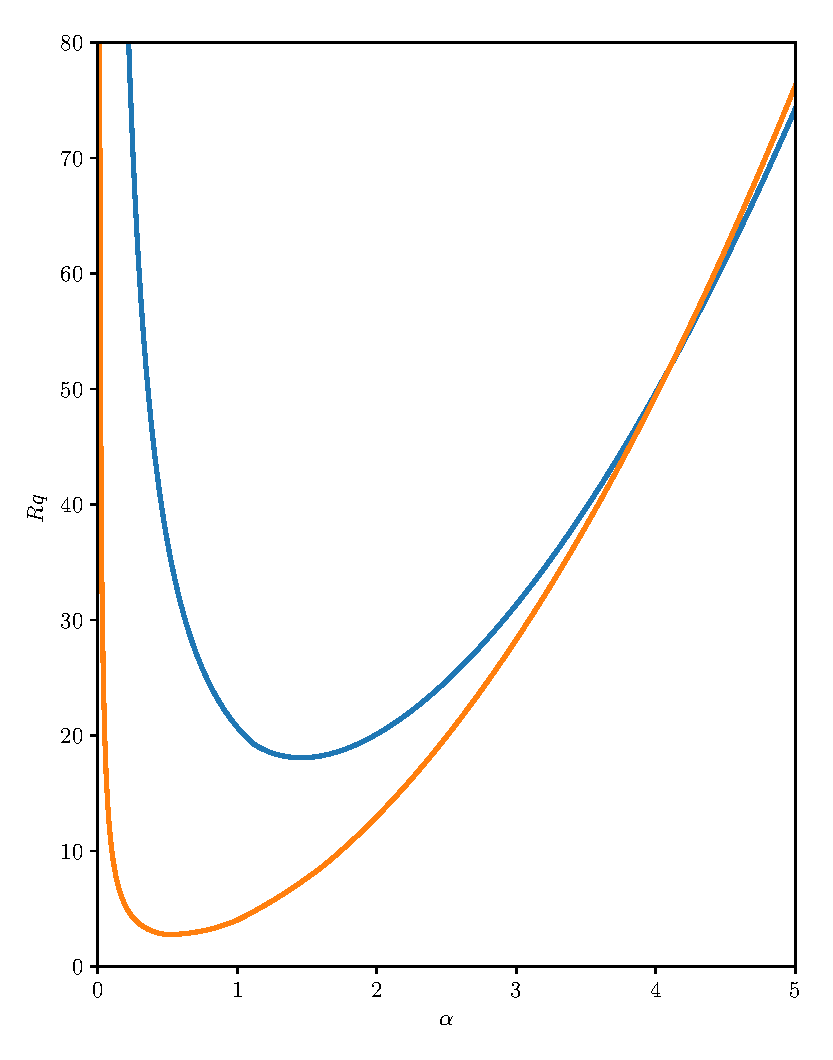
\includegraphics[width=75mm]{figures/josephvsynge.eps}
    \caption{A comparison of the bounds given by Synge \eqref{sbounds} (orange line) vs the bounds given by Joseph \eqref{jbound} (blue line)}
    \label{fig:josephvsynge}
\end{figure}

In real life, we wouldn't expect a flow to be modelled by just one wave number, meaning that for a flow to be stable, it must be so for all wavenumbers. This means that these bounds predict the existence of a \emph{critical Reynolds number}, found at the minimum point on this curve. The critical Reynolds number is the value of $R$ above which we see instability. Synge's bound has a minimum point at $ Rq = 2.74 $, $\al = 0.50 $. For Poiseuille flow, this corresponds to a critical $R$ value of $ 1.37 $, whereas, for Couette flow, this corresponds to a critical value of $ 2.74 $ (recall that $ q = 2 $ for Poiseuille flow and $ q = 1 $ for Couette flow). Joseph's bounds predict a significantly higher critical $R$ value of roughly $ 9.03 $ for Poiseuille flow and around $ 18.06 $ for Couette flow at $ \al = 1.46 $. These results predict that only flows with very low $R$ will be stable and that Couette flow is more stable than Poiseuille flow. Notice that the more accurate bound (of Joseph) has a higher critical $R$ value and a larger area of certain stability, implying that a more accurate curve may have an even higher critical $R$ value and a larger area of certain stability. 

These methods provide a bound on stability. However, they required a large number of significant approximations to derive and as such we wouldn't expect them to be very accurate. We also cannot get the values of specific eigenvalues for a flow, and it isn't easy to check whether a flow with a given $ R $ and $ \al$ is stable. For this reason, we turn to a numerical method that will allow us to obtain these results along with a more accurate curve of marginal stability. The next chapter introduces the numerical method we will be using.






